\documentclass[a4paper,utf8]{article}
\usepackage[heading,fancyhdr]{ctex}
\usepackage{amsmath,amssymb,geometry,lastpage,ulem}
\usepackage{array,tabularx,graphicx}
\geometry{
    top=25.4mm, 
    left=30mm, 
    right=30mm, 
    bottom=35mm,
    headsep=5.9mm,
}
\ctexset{
    section = {format+=\raggedright}
}
\newcommand{\expinfo}[5]{
    {\zihao{-3}\bfseries\songti
    实验名称:\uline{\hfill\mbox{#1}\hfill} \\[2.9mm]
    学\quad 号:\uline{\makebox[25mm]{#2}}\hfill
    姓\quad 名:\uline{\makebox[25mm]{#3}}\hfill
    班\quad 级:\uline{\makebox[25mm]{#4}} \\[2.9mm]
    合作者:\uline{\makebox[25mm]{无}}\enspace~
    桌\quad号:\uline{\makebox[25mm]{}}\hfill\mbox{}\\[2.9mm]
    指导教师:\uline{\makebox[30mm]{#5}}\hfill\mbox{} \\[2.9mm]
    实验日期:\uline{\makebox[30mm]{}}\hfill\mbox{} \\[58.7mm]
    }
}%\expinfo{实验名称}{学号}{姓名}{班级}{指导教师}
\pagestyle{fancy}
\fancyhf{} \fancyhead[C]{材料科学基础实验} \fancyfoot[C]{\thepage~/~\pageref{LastPage}}
\begin{document}
\begin{center}
    {\mbox{}\\[7em]\zihao{2}\bfseries\songti%
    材料科学基础实验报告}\\[34mm]
    \expinfo{实验二  金相试样的制备}{22301070}{杨雨燃}{22材物}{杨玉华}
\end{center}
\newpage
\section*{【实验目的】}
    \begin{enumerate}
        \item 了解金相分析基本概念。
        \item 掌握碳钢金相试样的制备方法及显微组织的显示方法。
        \item 按金相试样流程制备1个碳钢金相试样,并观察和分析其显微组织。
    \end{enumerate}   
\section*{【实验原理】}%简单描述,含必要的公式和附图;
\textbf{(一) 金相分析}

金相分析是研究金属材料内部组织和缺陷的最重要的方法。

进行金相分析,首先应根据各种检验标准和规定进行试样制备。若试样制备不当
,则可能出现假象,从而得出错误的结论。因此,金相试样的制备是金相分析的关键
,同时,从事金相分析的人员,须具备一定的热
处理基础知识,了解和熟悉常用金属材料在不同方式热处理下的相组成和组织组成。

\textbf{(二)晶相试样的制备}

金相试样的制备包括试样的截取、镶嵌、磨制、抛光及浸蚀等几个步骤,最终试
样需达到于显微镜下可观察到其真实组织,无磨痕、拖尾、麻点、水渍,并使金属中
夹杂物、石墨等不脱落等要求。
    \begin{enumerate}
        \item 金相试样的截取,金相试样一般制成边长为10mm的立方体,或直径10~15mm,高 10~18mm圆柱体,按实际情况有时制成片状、丝状或不规则形状的。金相试样截取试样的方法很多,根据零件大小、材料性能、现场实际情况选择。
        
        \item 金相试样的镶嵌,镶嵌这一工序并非是制备所有金相试样都必须进行的,具有前述形状及大小的试样,可直接进行磨光,但对于线材、细小的管材薄板以及形状不规则的小试样,磨光操作时极为不方便,这就需要用镶嵌的方法把它们镶嵌成便于操作的较大的试样,常用的镶嵌法主要有低熔点合金镶嵌法、塑料镶嵌法、机械镶嵌法等。

        \item 金相试样的磨光 ,若所选的观察面很不平整时,则需先用锉(对软金属)或砂轮(对硬金属)磨平,然后进行磨光。
        磨光分为粗摩和细摩。粗摩的目的是平整试样表面,同时去除掉截取试样所产生的应力变形层,为细磨做准备。磨光的第一个步骤应对试样磨面的边缘进行倒角,以防后道工序中,尖角、棱角划破砂纸及抛光布,甚至划伤手指。经粗磨后的试样表面虽较平整,但仍存在有较深的磨痕。细磨的目的就是为了消除这些磨痕,得到平整而光滑的磨面,并为进一步的抛光做好准备。
        
        手工磨光:手工磨光是在由粗到细的各号金相砂纸上进行。砂纸上的磨料一般是碳化硅或氧化铝微粉。砂纸平铺在玻璃、金属、塑料或木板等光滑平板上,
        磨制过程中操作人员需一手紧压砂纸,另一手平稳地拿住试样,将磨面轻压砂纸,向前平推,然后提起、拉回,拉回时试样勿与砂纸接触,
        不可来回磨削,否则磨面易成弧形,不易得到平整的磨面。手工磨光是用各号砂纸由粗到细而进行。
        手工磨光所需砂纸如下表。

        \begin{center}
            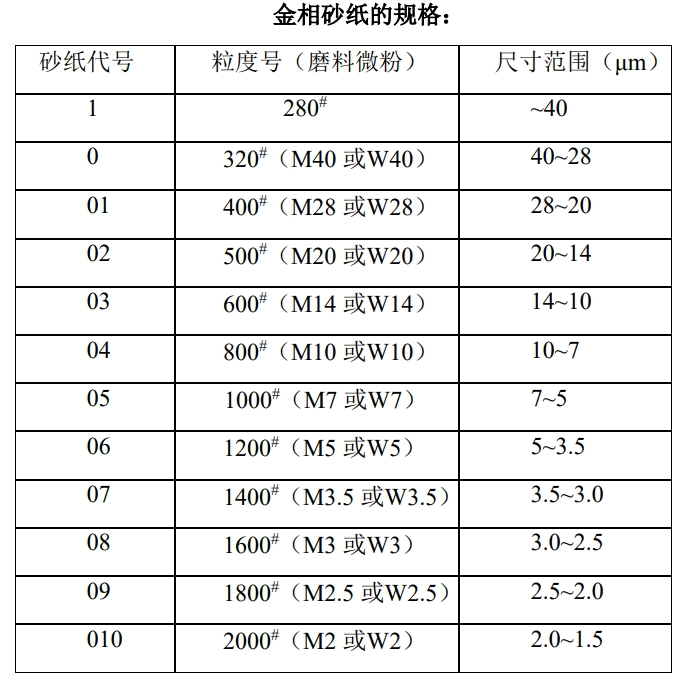
\includegraphics[width=400pt]{1.png}
        \end{center}

        \item 金相试样的抛光, 
        抛光的目的是为了清除最细一号砂纸磨光后试详表面所留下的细微磨痕,使试样
        的磨面成为光滑无痕的镜面。抛光操作时应注意以下事项: 
        
        (1) 抛光之前必须仔细检查磨面,当磨面上只留有单一方向的均匀的细磨痕时,才
        能进行抛光,以免徒劳往返,白费时间。

        (2) 抛光时,断断续续地加入抛光液或抛光膏于抛光织物上,抛光织物必须保持一定的
        润湿度,这对抛光结果影响很大。若织物过湿,能使钢中的非金属夹杂物及铸铁中的石
        墨脱出;若织物过干,则抛光的润滑作用较差,磨面将变得晦暗而有墨斑,对于较软试
        样有拖伤磨面的可能,以致影响对结果的判断。在抛光过程中,抛光织物上的磨料与水
        分逐渐散失,因此应随时加以补充,关于究竟保持怎样的润湿度最为理想,不同的试样
        ,不同的操作人员与操作方式情况下,需要经过一定的实践掌握自己的规律。

        (3) 转盘的速度要恰当,转速过高,磨料容易散失,转速过低影响抛光效果。对于软
        金属试样,转速应低一些,对硬金属试样,转速可高一些。一般在400-500转/分的范
        围内,也有低至100 转/分和高达1400 转/分的。

        (4) 抛光时手握试样,使磨面均匀地轻压在转盘上,若压力大而不均,会使表层金属
        变形,且试样易脱手飞出。抛光初期,试样最好保持在这样的位置,使转盘旋转的方向
        与最后一道磨光工序所留下的磨痕方向相垂直,以便于观察磨光是否完全消除,同时要
        将试样在转盘上沿半径方向由中心至边缘往复移动,使试样各部分抛光程度一致。在抛
        光的最后阶段,应将试样逆着圆盘旋转方向缓慢转动,以防止非金属夹杂物脱出和在磨
        面上产生如慧星尾巴状的痕迹。

        (5) 抛光时间不宜过长,长时间的抛光不但不能消除较粗的划痕,反而会使组织组成
        物着色,并严重扰乱金属组织层。

        \item 金相显微组织的显示,试样抛光后,其磨面在显微镜下仅呈光亮的一片,因此需要另外的操作使金相组织显示出来,最常用的是化学浸蚀法和电解侵蚀法。
        
        化学浸蚀操作:磨面在浸蚀前必须冲洗清洁,用酒精去除油污,以免阻碍浸蚀。浸蚀操作有两种方法:浸入法及擦拭法。我们采用擦拭法,即用蘸有浸蚀剂的棉花在磨面上轻轻擦拭,因为一般浸蚀的时间都很短,用这种方法比较容易控制,擦拭动作要迅速,并注意观察磨面上光泽的变化,浸蚀时间的长短随浸蚀剂及试样而不同,要视具体情况而定,浸蚀好后,要立即用洒精擦拭并吹干,然后进行显微观察。

        若显微组织没有完全显示出来,必然是浸蚀过浅,可再继续浸蚀;如果组织色调过于灰黑,失去应用的衬度,则为浸蚀过度,纠正的方法是重新抛光,甚至再用细号砂纸重磨;
        
        如果浸蚀后组织模糊不清,不能代表合金的正常组织,这说明磨面表层的非晶形层仍然存在,需经多次洗涤抛光浸蚀,交替操作以除去之。
    \end{enumerate}


\section*{【实验仪器】}%规格及参数
MDS400 金相显微镜、金相预磨机、金相抛光机、金相砂纸、玻璃板、抛光膏、4% 硝
酸酒精、75%酒精、吹风筒、脱指棉球、竹镊子等。
\section*{【实验过程】}%简述主要过程和实验内容

1. 领取试样、并选择不同型号砂纸共6张;

2. 磨光

3. 抛光

4. 浸蚀

5. 在金相显微镜下检查所制备的金相试样的质量。


\section*{【实验数据】}
简单的形貌分析:


最后的金相图片如下:



\end{document}